% Name: Cache hierarchy
% Description: A four-core processor with private L1 and L2 caches, a shared L3, and main memory, with typical sizes and access times beside each level.
% Tags: cache, memory hierarchy, CPU, computer architecture

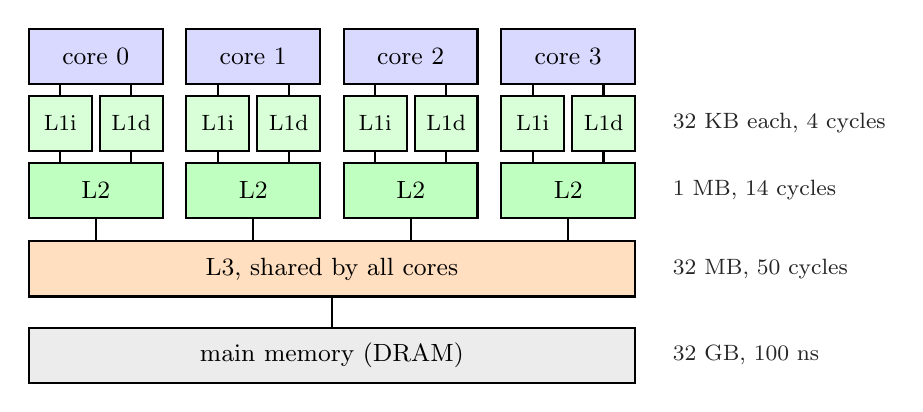
\begin{tikzpicture}[every node/.style={font=\small}, thick,
    box/.style={draw, minimum height=7mm, inner sep=1pt}]
  \foreach \i in {0,...,3} {
    \node[box, fill=blue!15, minimum width=17mm] at (2*\i,0) {core \i};
    \node[box, fill=green!15, minimum width=8mm, font=\footnotesize] at (2*\i-0.45,-0.85) {L1i};
    \node[box, fill=green!15, minimum width=8mm, font=\footnotesize] at (2*\i+0.45,-0.85) {L1d};
    \node[box, fill=green!25, minimum width=17mm] at (2*\i,-1.7) {L2};
    \draw (2*\i-0.45,-0.35) -- (2*\i-0.45,-0.5) (2*\i+0.45,-0.35) -- (2*\i+0.45,-0.5) (2*\i-0.45,-1.2) -- (2*\i-0.45,-1.35) (2*\i+0.45,-1.2) -- (2*\i+0.45,-1.35) (2*\i,-2.05) -- (2*\i,-2.35);
  }
  \node[box, fill=orange!25, minimum width=77mm] at (3,-2.7) {L3, shared by all cores};
  \draw (3,-3.05) -- (3,-3.45);
  \node[box, fill=gray!15, minimum width=77mm] at (3,-3.8) {main memory (DRAM)};
  % Typical figures for a recent desktop processor.
  \foreach \y/\t in {-0.85/{32 KB each, 4 cycles}, -1.7/{1 MB, 14 cycles}, -2.7/{32 MB, 50 cycles}, -3.8/{32 GB, 100 ns}}
    \node[anchor=west, gray!30!black, font=\footnotesize] at (7.2,\y) {\t};
\end{tikzpicture}
